\chapter{总体设计}
\section{软件描述}
系统包括前台和后台两个部分。

前台主要功能是:初始化界面的显示、关操作的请求(如输入用户名密码等)、用户的文件相关操作的请求(如选中文件并上传、下载、分享等操作)的控制信息的发送以及数据文件的发送、用户操作的结果显示等。

后台主要功能是:处理用户的输入,判断其权限、其操作是否合法;对于相应的文件操作,进行相应的判断与处理,比如:对于上传以及分享的文件,进行内容审核处理;对文件进行存储冗余处理;并且将处理结果(包括操作的结果以及下载操作对应的数据文件的发送等)返回到客户端。

\section{处理流程}
\subsection{总体流程}
总体流程图如图3.1所示。总体上来说,客户端将用户的请求通过网络发送到服务器端,服务器端对该请求进行检查,审核等处理之后,再执行相关操作,并最终将操作的结果返回到客户端。
\begin{figure}[!ht] 
\centering
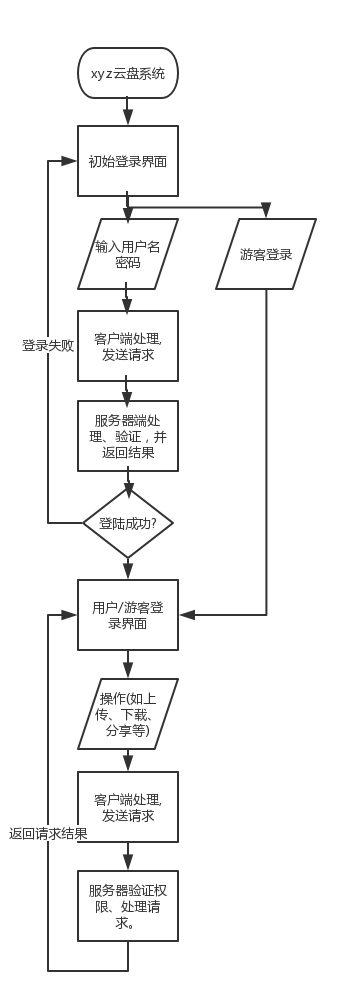
\includegraphics[width=7cm]{flow_overall.png} 
\caption{总体流程图}\label{fig:noted-figure}
\end{figure}

\subsection{系统基本流程} 
系统基本流程如图3.2所示。
\begin{figure}[!ht] 
\centering
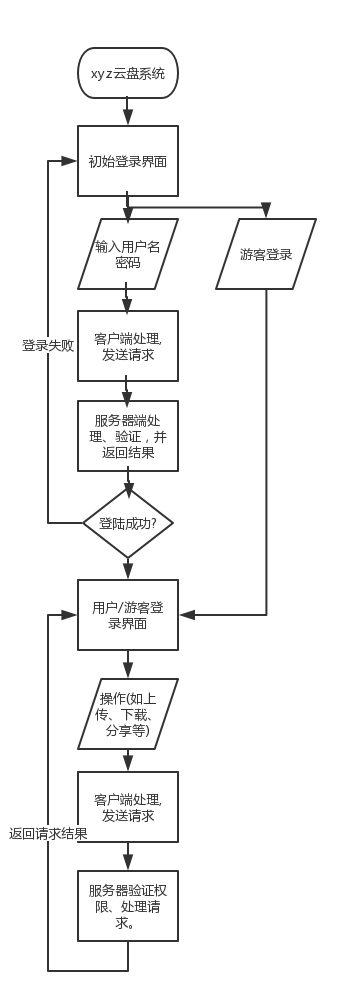
\includegraphics[width=7cm]{flow_system.png}
\caption{系统基本流程图}\label{fig:noted-figure}
\end{figure} 


\subsection{客户端基本流程}
客户端基本流程如图3.3所示。
\begin{figure}[!ht] 
\centering
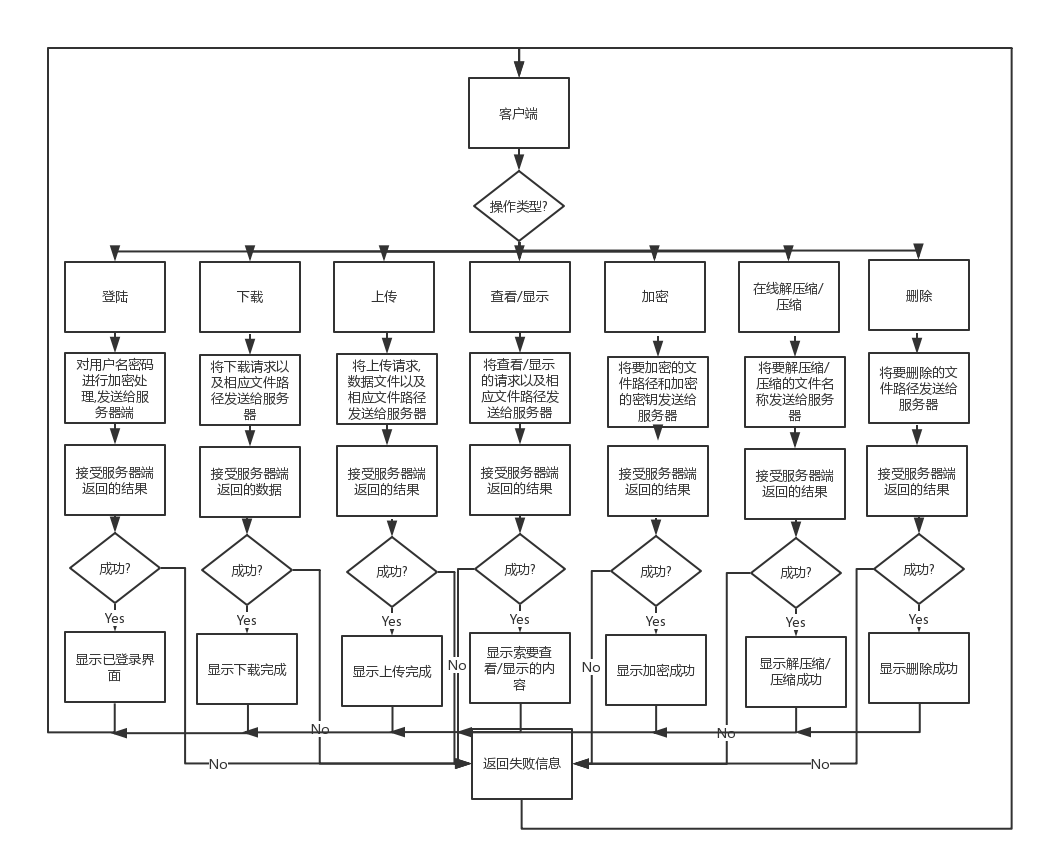
\includegraphics[width=18cm]{flow_client.png}
\caption{客户端基本流程图}\label{fig:noted-figure}
\end{figure}

\subsection{服务器端基本流程}
服务器端基本流程如图3.4所示。
\begin{figure}[!ht] 
\centering
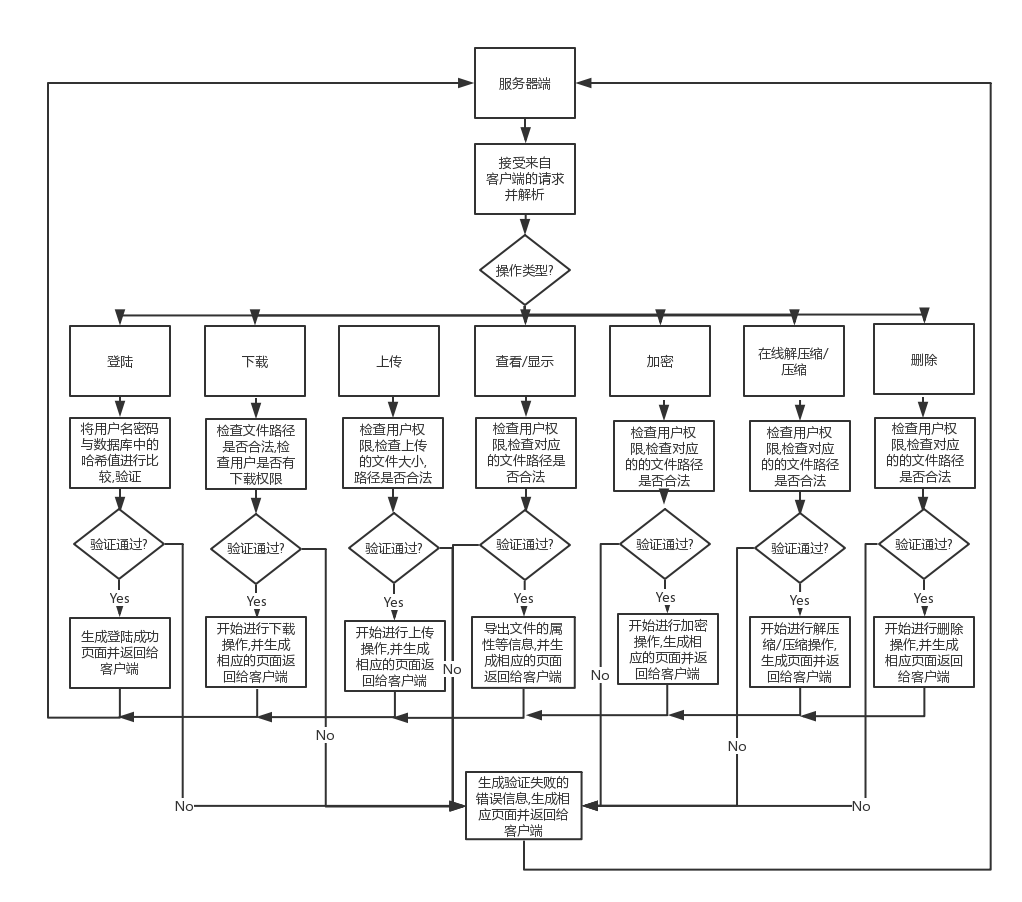
\includegraphics[width=18cm]{flow_server.png}
\caption{服务器端基本流程图}\label{fig:noted-figure}
\end{figure} 



\subsection{功能1-用户登录的具体流程} 

用户在初始登录界面输入用户名和密码。

在点击登录按钮之后,客户端检测用户名和密码的长度以及字符是否符合要求,如果不合法则弹出“用户名和密码违法”的界面;否则客户端将用户名和密码结合时间戳进行密码学处理并发送到服务器端。

服务器端通过密码学处理比对数据库中的用户信息,如果密码正确,返回带有时间戳的cookie给客户端。

客户端收到之后,如果密码正确,生成HTML页面,显示用户的根文件夹;如果密码错误,生成HTML页面,显示“密码错误”,以及错误次数,进行警告。

\subsection{功能2-用户注册的具体流程}

在看到登陆界面之后,用户可以点击“注册”键。客户端生成HTML页面,跳转到注册页面。之后在新的页面中用户输入用户名和绑定邮箱以及密码,点击“确认”键。

客户端检查用户名密码的字符以及长度是否符合要求,如果不符合要求,则生成HTML页面,提示“不符合要求”;否则将用户名密码以及绑定邮箱,结合时间戳进行密码学处理之后打包,通过POST发送给服务器端。

服务器端通过密码学手段验证用户名和邮箱是否有效。如果无冲突且有效,在服务器端创建新用户,并设置对应的邮箱一直处理后的密码。如果冲突或者无效,则返回错误信息给客户端。

如果注册成功,客户端生成HTML页面,提示成功;如果用户名或邮箱冲突或无效,则生成HTML页面,显示相应信息。

\subsection{功能3-用户忘记密码的具体流程}
在看到登陆界面之后,用户可以点击“忘记密码”键,客户端生成HTML页面,,跳转到新页面。之后在新的页面中输入绑定邮箱以及新的密码,点击“确认”键。

客户端将密码和邮箱,结合时间戳进行密码学处理之后打包,通过POST发送给服务器端。

服务器端检查邮箱是否有效。如果邮箱对应的用户存在,则生成随机链接到对应邮箱中,以便重置密码,并返回“邮箱已发送”信息给客户端。如果不存在用户,则返回“邮箱不存在”给客户端。

如果服务器在规定时间(15min)内收到该链接下的新的密码,则修改该用户的密码为新密码。

如果客户端收到“邮箱已发送”,则显示“邮箱已发送”;如果客户端收到“邮箱不存在”,则显示“优先不存在”。

\subsection{功能4-上传文件的具体流程}

用户点击“上传”按钮,在弹出的对话框中选择所要上传的文件或文件夹,并点击“上传”按钮。

客户端在用户第一次点击“上传”按钮时,显示小型资源管理器以便查找。在用户第二次点击“上传”按钮之后,客户端与服务器建立tcp链接,开始上传。上传时根据传输情况,计算速度,剩余时间,进度,剩余文件大小等信息。

客户端在用户第一次点击“上传”按钮时,弹出小型资源管理器。在用户第二次点击“上传”按钮之后,显示开始上传。上传时显示速度,剩余时间,进度,剩余文件大小等信息。


\subsection{功能5-下载文件的具体流程}

用户选中所要下载的文件以及文件夹,点击“下载”按钮,在弹出的对话框中选择所要存储的文件夹,并点击“下载”按钮。

客户端在用户第一次点击“下载”按钮时,显示小型资源管理器以便设置下载路径。在用户第二次点击“下载”按钮之后,客户端与服务器建立tcp链接,开始下载。下载时根据传输情况,计算速度,剩余时间,进度,剩余文件大小等信息。

客户端在用户第一次点击“下载”按钮时,弹出小型资源管理器。在用户第二次点击“下载”按钮之后,显示开始下载。下载时显示速度,剩余时间,进度,剩余文件大小等信息。

\subsection{功能6-新建文件夹的具体流程}
用户在当前目录空白处右键点击新建文件夹,或在点击新建文件夹的功能按钮,在窗口输入名称并点击确认

客户端将新建文件夹的指令与名称打包发给服务端,服务端首先检查名字是否有效,否则提示非法名称,是则判断文件夹是否已经存在,是则创建,否则返回名称冲突的错误。

若创建成功,则刷新当前目录,否则输出错误信息


\subsection{功能7-打开文件夹的具体流程}
用户双击文件夹,或者选中文件夹之后点击打开选项。

客户端将打开文件夹的指令打包,发送到服务器,服务器传回文件夹内容。客户端接收之后,切换路径到所选中的文件夹,并展示其所包含的文件及文件夹。

若无异常发生,客户端显示文件夹中的文件以及子文件夹。


\subsection{功能8-重命名的具体流程}
用户选中文件或文件名,右键,选中“重命名”选项。

客户端将重命名的原名字和新名字打包发给服务器端。

服务器检查该重命名是否合法不冲突,是则返回“成功”的信息,否则,返回“失败”的信息。

如果成功,则刷新当前目录,显示最新的名字。如果失败,则提示失败。


\subsection{功能9-复制、粘贴、剪切的具体流程}
复制:用户选中需要操作的文件和文件夹,右键,选中“复制”选项。客户端将用户选中要复制的项的完全名字(包括路径)存储到cache中。

剪切:用户选中需要操作的文件和文件夹,右键,选中“剪切”选项。客户端将用户选中要剪切的项的完全名字(包括路径)存储到cache中。

粘贴:用户在所要粘贴的文件夹中,右键,选中“粘贴”选项。需要注意的是,必须有之前“复制”或“剪切”的操作记录,“粘贴”选项才可选。客户端将执行粘贴的文件夹的路径,以及之前复制或者剪切的类型一起打包,发给服务器端。服务器接收之后检查命名是否冲突。如果冲突就返回“命名冲突”信息;如果不冲突,如果是复制,则复制到目标文件夹,如果是剪切,则先复制,再删除。最后返回“成功”给客户端

如果粘贴成功,则刷新当前文件夹,显示最新结果。
如果粘贴失败,则弹窗提示粘贴失败。

\subsection{功能10-移入回收站、移出回收站、彻底删除的具体流程}
移入回收站:

用户选中文件或文件夹,右键,选中“移入回收站”选项。客户端将该文件或文件夹名字(包括路径)打包发送到服务器端。服务器将该文件或文件夹移入“回收站”中并返回“成功”。客户端收到信息后,刷新当前文件夹。

 
移出回收站:

用户在回收站中选中文件或文件夹,右键,选中“移出回收站”选项。
客户端将该文件或文件夹名字(包括路径)打包发送到服务器端。服务器端检查该文件或文件夹复原之后是否有命名冲突等。如果无冲突则移出“回收站”中并返回“成功”,否则返回“失败”。客户端收到信息后,如果成功,则刷新回收站;如果失败,则弹窗提示。

彻底删除:

用户在回收站中选中文件或文件夹,右键,选中“彻底删除”。
客户端将该文件或文件夹名字(包括路径)打包发送到服务器端。服务器从回收站中删除。返回“成功”。客户端收到信息后,如果成功,则刷新回收站;如果失败,则弹窗提示。


\subsection{功能11-加入收藏夹、移出收藏夹的具体流程}
加入收藏夹:

用户选中文件或文件名,右键,选中“加入收藏夹”选项。
客户端将用户选中的文件名打包发给服务器端,服务器将该文件或文件夹加入所维护的收藏夹数据结构中。返回成功。

移出收藏夹:

用户在收藏夹中选中文件或文件名,右键,选中“移出收藏夹”选项。
客户端将用户选中的文件名打包发给服务器端,服务器将该文件或文件夹从所维护的收藏夹数据结构中删除。返回成功。

\subsection{功能12-加密的具体流程}
用户选中所要加密的文件或文件夹,右键,选中“加密”选项。在接下来弹出的对话框中写入不同于登录密码的密钥。

客户端将用户输入的密钥进行密码学处理,和对应的文件以及文件夹名称一起打包,发给服务器。服务器端用对该文件及文件夹设置加密标记,并保存经密码学处理的密钥,以便后面比对。最后服务器将陈工信息返回给客户端。

如果成功,则提示加密成功。否则弹窗提示失败。



\subsection{功能13-分享的具体流程}
用户选中所要分享的文件或文件夹,右键,如果选中“分享”选项。接下来会生成带有随机字符串的链接。用户将该字符串发送给其他用户。

用户在客户端点击“导入分享”按钮,在弹出的对话框中输入链接;也可以直接用该链接用其他软件下载。

客户端在用户点击“分享”之后,将文件或文件夹的名字(包括路径)打包,标记“分享”发通过POST送给服务器端。服务器收到后根据路径名生成带有随机字符串的链接,发送给客户端。服务器维护文件名字到链接的映射,以便分享,以及在规定时间之后(如七天)取消该链接有效性。

在其他用户点击”导入分享“之后,客户端将该链接发送到服务器端。服务器检查该串是否有效,如果无效则返回”无效“给客户端;否则在服务器中将该文件或文件夹复制到该用户空间中,返回”成功“给客户端。

客户端在用户点击“分享”之后,如果成功,则提示成功,并显示该链接;否则提示失败。

其他用户在导入时,如果链接无效则提示无效,否则提示成功,并刷新页面,显示该文件或文件夹的位置。

\subsection{功能14-搜索的具体流程}
用户在当前目录上方的搜索框输入关键字,点击搜索

客户端将当前目录与关键字打包发送到服务器,服务器对当前目录与子目录的文件、文件夹列表以及可见的共享文件夹进行匹配,返回匹配成功的列表。

客户端像进入一个新的文件夹一样显示搜索结果

\subsection{功能15-预览的具体流程}
用户不做显式的操作

服务器将当前目录的文件进行格式匹配:

1. 文档,在大图标模式下,返回第一页的图片;在小图标模式下,返回对应格式的图标

2. 视频:在大图标模式下,返回随机帧的秃瓢;在小图标模式下,返回对应格式的图标

3. 其他文件:返回该文件附带的图标,若无则返回对应格式的图标

显示文件列表时显示对应的图标或预览

\subsection{功能16-在线解压/压缩的具体流程}
解压:

用户在一个压缩文件上右击,点击在线解压

客户端将文件路径与解压指令发送给服务端,服务器查找文件是否存在且为压缩文件:
1. 查找成功,尝试解压。若成功,则解压到同名文件夹(若同名文件夹已存在,则解压入内),否则生成HTML页面,提示解压失败
2. 查找不成功,生成HTML页面,提示文件不存在

压缩:

用户在当前文件夹复选多个文件、文件夹,单机压缩功能按钮或右键选择压缩,点击确认或更改默认压缩文件名后点击确认。

客户端提示的默认压缩包名为:若只选择了一个文件、文件夹,则压缩包名称默认为它的名字。
若选择了多个文件、文件夹,则压缩包名称默认为当前目录的名字(若当前目录为用户网盘根目录,则为用户名称)。

客户端将复选的文件与压缩指令、压缩包名称发送给服务端。
服务端确认这些文件的存在,并根据压缩包名称创建压缩文件:若名称冲突,则在其后增加"(1)"(若仍冲突则改为"(2)",类推)
压缩成功后,生成HTML页面,提示压缩成功


\subsection{功能17-举报的具体流程}
用户选中所要举报的文件以及文件夹,右键,选择“举报”选项。在接下来弹出的对话框中选择举报的分类。

客户端在用户点击“举报”选项之后,生成对话框,之后将用户所选择的文件以及文件夹的名字以及举报类型打包,发给服务器端。

服务器接收之后记录文件名,及其md5值,并在所维护的举报库中找到相应md5,如果找到了,就增加举报次数,如果没有找到则将md5值与文件信息加入,并设置举报次数为1。
最后服务器端返回成功信息给客户端。

运维人员定期检查举报库,判断文件是否应被屏蔽。若是,则将举报库中该条文件设为已审核,屏蔽。否则,将该条文件设为已审核,放行。

客户端生成HTML页面,显示”感谢您的举报“窗口。

\subsection{功能18-审核的具体流程}
用户对网盘文件进行正常的修改操作

服务器对每次目录的更新(重命名,添加文件/文件夹)进行匹配文件名,若关键字匹配成功,则使该次修改操作失败,并返回错误信息:敏感关键字。

服务器对文件的更新(上传,粘贴移动)进行md5匹配,若在举报库中匹配md5成功且该文件未屏蔽状态,则使该次操作失败生成HTML页面,并返回错误信息:该文件已被举报。


\subsection{功能19-标签页创建/关闭的具体流程}
创建:

用户点击标签页旁边的创建按钮。

客户端打包指令发送给服务端,服务端返回与当前目录相同的一个子页面作为新的标签页。

用户在标签页栏看到与当前标签页在同一目录的新标签页。

关闭:

用户点击标签页上的关闭按钮。 

客户端打包指令发送给服务端并删除该子页,服务端返结束该会话记录。

该标签页被关闭,从标签栏中消失。 

\subsection{功能20-创建共享文件夹的具体流程}

用户点击“创建共享文件夹”按钮,输入想要创建的共享文件夹的名称,选择想要对其可见的用户列表,并对其分配权限:管理,读,写

用户点击创建并输入文件夹名后,客户端将相关指令信息打包发送给服务端

服务端在专门设置的放置共享文件夹的位置创建该文件夹。若创建失败,则返回错误信息。若创建成功,则根据用户设置的权限对文件夹的属性进行修改。

客户端收到创建成功或失败,显示提示信息。

\subsection{功能21-进入共享文件夹的具体流程}

用户点击共享文件夹按钮,客户端将此命令打包发送到服务器。
                                                                             
服务器传回所有对用户可见的共享文件夹(看起来就像此时进入了一个文件夹一样)。

用户点击想要进入的共享文件夹,客户端将指令打包发送到服务器

服务器传回该共享文件夹内的所有对该用户的可见文件,从而进入了该文件夹。之后的操作与普通文件夹一样,但多了一个额外限制:只返回对改用户可见的文件。

用户选择进入一个共享文件夹,之后对其的操作与普通文件夹一样

\subsection{功能22-共享文件夹的权限匹配的具体流程}

用户对共享文件夹/其中的文件夹、文件进行像普通文件(夹)一样的操作:修改权限,创建文件夹、文件,下载,上传,重命名,删除,移动,复制粘贴,预览

客户端的行为与普通文件夹下的行为一致,但在服务端需要判断用户的权限是否允许客户进行该操作:

用户需要有该文件的读权限:

1. 下载

2. 复制、移动到用户个人网盘

3. 预览

用户需要有该文件的写权限:

1. 删除

2. 重命名

3. 移动

4. 上传对其进行覆盖

5. 删除的文件夹内包含这个文件

用户需要拥有该文件夹的读权限:

1. 进入该文件夹

2. 下载该文件夹

3. 复制、移动到用户个人网盘

4. 预览

用户需要有该文件夹的写权限:

1. 向其中上传文件(夹)

2. 在其中删除文件(夹)

3. 重命名该文件夹

4. 移动该文件夹

5. 上传文件夹对其进行合并

6. 删除该文件夹

7. 删除该文件夹所属的文件夹

用户需要有该共享文件夹的管理权限:

1. 修改其内文件、文件夹的权限分配

2. 移除该共享文件夹

若服务端发现用户指令与其权限不匹配,返回权限不匹配的信息,否则正常进行操作并返回正常操作的返回信息

\subsection{功能23-共享文件夹的权限管理的具体流程}

用户对共享文件夹中的文件夹/文件或共享文件夹本身点击管理按钮,选择指定的用户并修改其对应的各个权限,点击确认

点击确认按钮后,客户端将指令打包发给服务端

服务端判断用户是否有管理权,若有则修改指令中的对应权限,并提示修改成功,否则,返回没有权限的错误信息

客户端根据返回信息提示修改是否成功



\section{功能结构设计}
\subsection{整体结构}
整体模块的结构如图3.5所示。整体结构由客户端的4个内部模块、1个外部模块,和服务器端的11个内部模块、1个外部模块组成。

\begin{figure}[!ht] 
\centering 
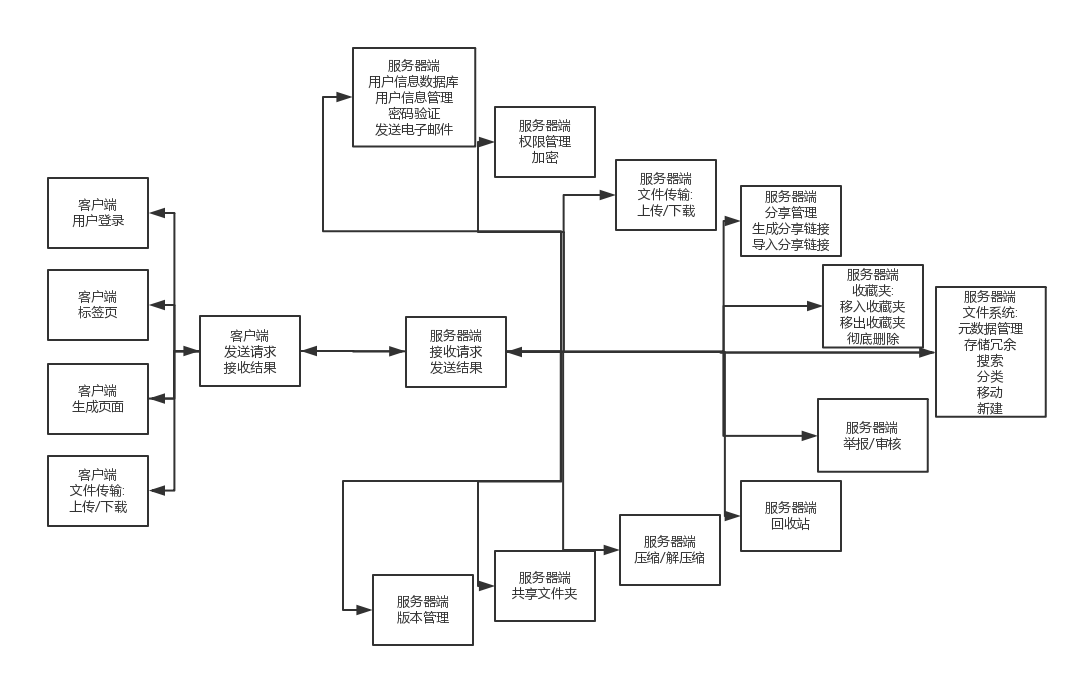
\includegraphics[width=18cm]{module_overall.png} 
\caption{整体结构模块图}\label{fig:noted-figure}
\end{figure}

\subsection{用户端结构}
用户端的模块结构如图3.6所示,
分成负责用户登录、注册、忘记密码的登陆模块,
负责标签页的创建与关闭操作的标签页模块,
负责生成页面,显示内容,弹出错误提示信息的显示模块,
负责上传文件、下载文件的传输模块,
以及与这些模块通信、与服务器端模块通信的通信模块一共5个模块构成。
\begin{figure}[!h]  
\centering 
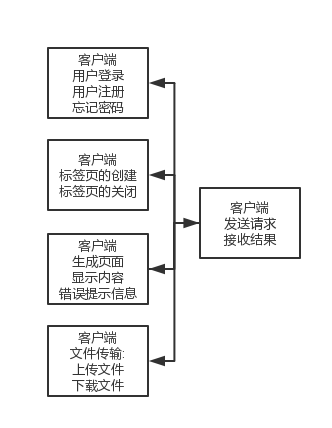
\includegraphics[width=8cm]{module_client.png} 
\caption{用户端模块结构图}\label{fig:noted-figure}
\end{figure}

\subsubsection{MODULE.CLIENT.1:通信模块}
将其他模块产生的输入打包为http请求,向服务器端发送,并将返回的内容传给该模块

\subsubsection{MODULE.CLIENT.2:登陆模块}
产生登陆页面。

若用户登陆,检查其用户名与密码合法性,将用户名与密码散列值传给通信模块,并解析返回的结果

若用户注册,则检查用户信息的合法性,并将其打包传给通信模块,解析返回的结果

若用户忘记密码,则检查用户信息的合法性,打包传给通信模块,解析传回的结果

\subsubsection{MODULE.CLIENT.3:标签页模块}
管理用户同时打开的多个标签页,对每个标签页有一个子页面。

将用户对标签的操作打包传给通信模块,解析传回的结果

\subsubsection{MODULE.CLIENT.4:显示模块}
绘制页面内容,包括文件列表、功能按钮、

\subsubsection{MODULE.CLIENT.5:传输模块}
t





\subsection{服务器端结构}
服务器端的模块结构如图3.6所示,
分成负责用户信息管理、密码验证、发送电子邮件等操作的用户信息数据库模块,
负责权限管理、文件加密的权限模块,
负责上传文件、下载文件的文件传输模块,
负责生成分享链接、导入分享链接的分享管理模块,
负责移入收藏夹、移出收藏夹的收藏夹模块,
负责文件元数据管理(如存储冗余、搜索、分类、新建、移动等)的元数据管理模块,
负责举办和审核的审核模块,
负责移入回收站、移出回收站、彻底删除的回收站模块,
负责压缩、解压缩的压缩模块,
负责共享文件夹操作的共享文件夹模块,
负责版本更新的版本管理模块,
以及负责与这些模块通信,
与客户端模块通信的通信模块,一共12个模块。

\begin{figure}[!h] 
\centering   
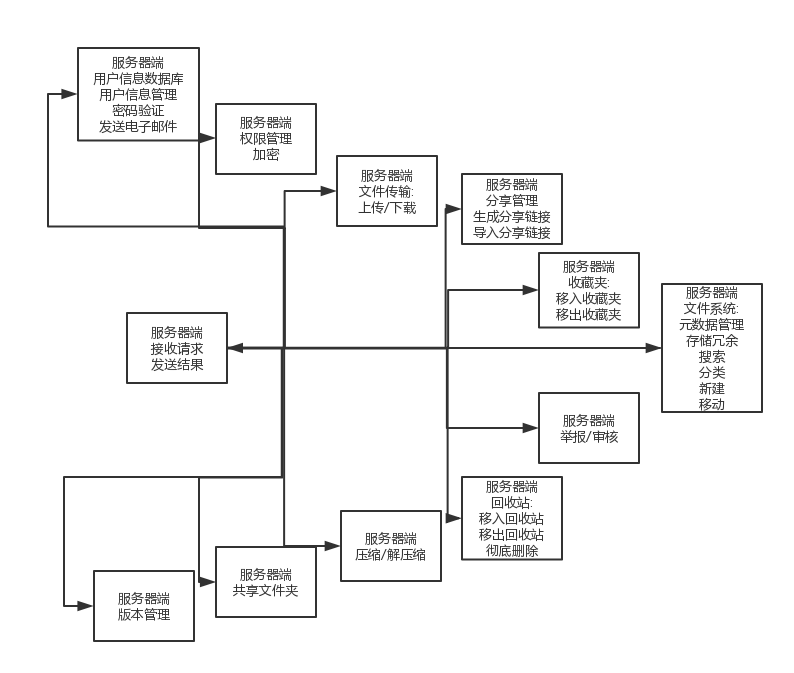
\includegraphics[width=16cm]{module_server.png}
\caption{服务器端模块结构图}\label{fig:noted-figure}
\end{figure}

\subsubsection{MODULE.SERVER.1:通信模块}
t

\subsubsection{MODULE.SERVER.2:用户信息数据库模块}
t

\subsubsection{MODULE.SERVER.3:权限模块}
t

\subsubsection{MODULE.SERVER.4:文件传输模块}
t

\subsubsection{MODULE.SERVER.5:分享管理模块}
t

\subsubsection{MODULE.SERVER.6:收藏夹模块}
t

\subsubsection{MODULE.SERVER.7:元数据管理模块}
t

\subsubsection{MODULE.SERVER.8:审核模块} 
t

\subsubsection{MODULE.SERVER.9:回收站模块}
t 

\subsubsection{MODULE.SERVER.10:压缩模块}
t

\subsubsection{MODULE.SERVER.11:共享文件夹模块}
t

\subsubsection{MODULE.SERVER.12:版本管理模块}
t






\section{功能需求与程序代码的关系}
这一小节分为功能需求与用户端代码的关系和功能需求与服务器端代码的关系两个部分。其中,与用户端代码的关系如表3.1,表3.2所示;与服务器端的代码的关系如表3.3,表3.4所示。
\begin{table}[!ht]
\centering
\caption{功能需求与程序代码的关系表1-用户端模块第1部分} \label{tab:requirement-module}
\begin{tabular}{|c|c|c|c|c|c|}
    \hline 
    需求ID & MD.CL.1 & MD.CL.2 & MD.CL.3 & MD.CL.4 & MD.CL.5 \\
    \hline 
    R..USER.LOGIN.001 &· &· &· & Y  &· \\
    \hline
    R..USER.LOGIN.002 & Y & Y &Y  &·  &· \\
    \hline 
    R..USER.LOGIN.003 & Y & Y & Y &·  &· \\
    \hline
    R..USER.LOGIN.004 & Y & Y & Y &·   &· \\
    \hline
    R..USER.LOGIN.005 &· &· &· & Y  &· \\
    \hline
    R..FILE.BASIC.001 & Y &· &· & Y  & Y \\
    \hline
    R..FILE.BASIC.002 & Y &· &· &  Y & Y \\
    \hline 
    R..FILE.BASIC.003 & Y  &·  & · &Y   &· \\
    \hline
    R..FILE.BASIC.004 & Y  &·  & · &Y  &· \\
    \hline
    R..FILE.BASIC.005 & Y  &·  & · &Y  &· \\
    \hline
    R..FILE.BASIC.006 & Y  &·  & · & Y  &· \\ 
    \hline
    R..FILE.BASIC.007 & Y  &·  & · & Y  &· \\
    \hline
    R..FILE.BASIC.008 & Y  &·  & · & Y  &· \\
    \hline
    R..FILE.BASIC.009 & Y  &·  & · & Y  &· \\ 
    \hline
    R..FILE.BASIC.010 &·  & · & Y & Y  &· \\ 
    \hline
    R..FILE.HIGH.001 & Y  &·  & · &Y  &· \\
    \hline
    R..FILE.HIGH.002 & Y  &·  & · & Y  &· \\
    \hline
    R..FILE.HIGH.003 & Y &· &· & Y  &· \\
    \hline
    R..FILE.HIGH.004 & Y &· &· &Y  &· \\
    \hline
    R..FILE.HIGH.005 & Y &· &· & Y  &· \\
    \hline
\end{tabular}
\note{表中的R..XXX等均指R.XYZ.CLOUDSTORAGE.XXX。   MD.CL指MODULE.CLIENT}
\end{table}

\begin{table}[!ht]
\centering
\caption{功能需求与程序代码的关系表1-用户端模块第2部分} \label{tab:requirement-module}
\begin{tabular}{|c|c|c|c|c|c|}
    \hline 
    需求ID & MD.CL.1 & MD.CL.2 & MD.CL.3 & MD.CL.4 & MD.CL.5 \\
    \hline 
    R..FILE.HIGH.006 &Y  &· &· &   Y& ·\\
    \hline
    R..FILE.HIGH.007 &Y  &·  &·  &  Y& ·\\
    \hline 
    R..FILE.HIGH.008 &Y  &·  &·  &  Y& ·\\
    \hline
    R..FILE.HIGH.009 &Y  &·  &·  &   Y& ·\\
    \hline
    R..FILE.HIGH.010 &Y &· &· &   Y& ·\\
    \hline
    R..FILE.HIGH.011 &Y  &· &· &   Y&  ·\\
    \hline
    R..TAB.001 &·  &· &Y &   Y&  ·\\
    \hline 
    R..TAB.002 &·   &Y  &·  &   Y& ·\\
    \hline
    R..SHAREFOLDER.001 &  Y &·  &·  &  Y& ·\\
    \hline
    R..SHAREFOLDER.002 &  Y &·  &·  &  Y& ·\\
    \hline
    R..SHAREFOLDER.003 &  Y &·  &·  &   Y& ·\\ 
    \hline
    R..SHAREFOLDER.004 &  Y &·  &·  &   Y& ·\\
    \hline
    R..VERSION.001 &  Y &·  &·  &   Y& ·\\
    \hline
\end{tabular}
\note{表中的R..XXX等均指R.XYZ.CLOUDSTORAGE.XXX。   MD.CL指MODULE.CLIENT}
\end{table}
 
\begin{table}[!ht]
\centering
\caption{功能需求与程序代码的关系表2-服务器端模块第1部分} \label{tab:requirement-module}
\begin{tabular}{|c|c|c|c|c|c|c|c|c|c|c|c|c|}
    \hline 
    需求ID & 1 & 2 & 3 & 4 & 5 & 6 & 7 & 8 & 9 & 10 & 11 & 12 \\    
    \hline 
    R..USER.LOGIN.001 &· &· &· &· &· &· &· &· &· &· &· &Y \\
    \hline
    R..USER.LOGIN.002 &Y&Y&· &· &· &· &· &· &· &· &· &  ·\\
    \hline 
    R..USER.LOGIN.003 &Y&Y&· &· &· &· &· &· &· &· &· &  ·\\
    \hline
    R..USER.LOGIN.004 &Y&Y&· &· &· &· &· &· &· &· &· &  ·\\
    \hline
    R..USER.LOGIN.005 &· &· &· &· &· &· &· &· &· &· &· &  ·\\
    \hline
    R..FILE.BASIC.001 &Y&· &Y&Y&· &· &Y&Y&· &· &· &  ·\\
    \hline
    R..FILE.BASIC.002 &Y&· &Y&Y&· &· &Y&Y&· &· &· &  ·\\
    \hline 
    R..FILE.BASIC.003 &Y&· &Y&· &· &· &Y&· &· &· &· &  ·\\
    \hline
    R..FILE.BASIC.004 &Y&· &Y&· &· &· &Y&· &· &· &· &  ·\\
    \hline
    R..FILE.BASIC.005 &Y&· &Y&· &· &· &Y&· &· &· &· &  ·\\
    \hline
    R..FILE.BASIC.006 &Y&· &Y&· &· &· &Y&· &· &· &· &  ·\\ 
    \hline
    R..FILE.BASIC.007 &Y&· &Y&· &· &· &Y&· &· &· &· &  ·\\
    \hline
    R..FILE.BASIC.008 &Y&· &Y&· &· &· &Y&· &· &Y&· &  ·\\
    \hline
    R..FILE.BASIC.009 &Y&· &Y&· &· &· &Y&· &· &Y&· &  ·\\ 
    \hline
    R..FILE.BASIC.010 &· &· &· &· &· &· &· &· &· &· &· &  ·\\ 
    \hline
    R..FILE.HIGH.001 &Y&· &Y&· &· &· &Y&· &Y&· &· &  ·\\
    \hline
    R..FILE.HIGH.002 &Y&· &Y&· &· &Y&Y&· &· &· &· &  ·\\
    \hline
    R..FILE.HIGH.003 &Y&· &Y&· &· &· &Y&· &· &· &· &  ·\\
    \hline
    R..FILE.HIGH.004 &Y&· &Y&· &Y&· &Y&Y&· &· &· &  ·\\
    \hline
    R..FILE.HIGH.005 &Y&· &Y&· &· &· &Y&· &· &· &· &  ·\\
    \hline
\end{tabular}
\note{表中的R..XXX等均指R.XYZ.CLOUDSTORAGE.XXX。第一行的1~12表示指MODULE.SERVER.1~12}
\end{table}

\begin{table}[!ht]
\centering
\caption{功能需求与程序代码的关系表2-服务器端模块第2部分} \label{tab:requirement-module}
\begin{tabular}{|c|c|c|c|c|c|c|c|c|c|c|c|c|}
    \hline 
    需求ID & 1 & 2 & 3 & 4 & 5 & 6 & 7 & 8 & 9 & 10 & 11 & 12 \\    
    \hline 
    R..FILE.HIGH.006 &Y&· &Y&· &· &· &Y&· &· &· &· &  ·\\
    \hline
    R..FILE.HIGH.007 &Y&· &Y&· &· &· &Y&· &· &· &· &  ·\\
    \hline 
    R..FILE.HIGH.008 &Y&· &Y&· &· &· &Y&· &· &· &· &  ·\\
    \hline
    R..FILE.HIGH.009 &Y&· &Y&· &· &· &Y&· &· &· &· &  ·\\
    \hline
    R..FILE.HIGH.010 &Y&· &Y&· &· &· &Y&Y&· &· &· &  ·\\
    \hline
    R..FILE.HIGH.011 &Y&· &Y&· &· &· &Y&Y&· &· &· &  ·\\
    \hline
    R..TAB.001 &· &· &· &· &· &· &· &· &· &· &· &  ·\\
    \hline 
    R..TAB.002 &· &· &· &· &· &· &· &· &· &· &· &  ·\\
    \hline
    R..SHAREFOLDER.001 &Y&· &Y&· &· &· &Y&· &· &· &Y&  ·\\
    \hline
    R..SHAREFOLDER.002 &Y&· &Y&· &· &· &Y&· &· &· &Y&  ·\\
    \hline
    R..SHAREFOLDER.003 &Y&· &Y&· &· &· &Y&· &· &· &Y&  ·\\ 
    \hline
    R..SHAREFOLDER.004 &Y&· &Y&· &· &· &Y&· &· &· &Y&  ·\\ 
    \hline
    R..VERSION.001 &Y&· &· &· &· &· &· &· &· &· &· &Y \\
    \hline
\end{tabular}
\note{表中的R..XXX等均指R.XYZ.CLOUDSTORAGE.XXX。第一行的1~12表示指MODULE.SERVER.1~12}
\end{table}
